\documentclass[14pt]{beamer}
\usepackage{fancyvrb}
\RecustomVerbatimCommand{\VerbatimInput}{VerbatimInput}{frame=single,
numbersep=1mm, numbers=left, formatcom=\color{orange}}
%\usepackage{kpfonts}
\usepackage[bitstream-charter]{mathdesign}
\usepackage[utf8]{inputenc}
\usepackage{pgf}
\usepackage{verbatim}
\usepackage[ruled,vlined,linesnumbered]{algorithm2e}
\usepackage{amsfonts,eucal}


\mode<presentation>
{


\usetheme{Boadilla}
\useoutertheme{split}
\usecolortheme{albatross}

\setbeamertemplate{blocks}[rounded][shadow=false]
\setbeamertemplate{navigation symbols}{}



\setbeamercolor*{structure}{fg=green!75!black,bg=blue!70!white}
\setbeamercolor*{normal text}{fg=green!65!black,bg=blue!80!black}
\setbeamercolor{palette primary}{use={structure,normal text},fg=green,bg=structure.bg!75!black}
\setbeamercolor{palette secondary}{use={structure,normal text},fg=structure.fg,bg=structure.bg!60!black}
\setbeamercolor{palette tertiary}{use={structure,normal text},fg=structure.fg,bg=structure.bg!45!black}
\setbeamercolor{palette quaternary}{use={structure,normal text},fg=green,bg=structure.bg!75!black}
\setbeamercolor*{example text}{fg=green!65!black}
\setbeamercolor*{block body}{bg=structure.bg!90!black}
\setbeamercolor*{block body alerted}{bg=structure.bg!90!black}
\setbeamercolor*{block body example}{bg=structure.bg!90!black}
\setbeamercolor*{block title}{parent=structure,bg=structure.bg!75!black}
\setbeamercolor*{block title alerted}{use={structure,alerted text},fg=alerted text.fg!75!structure.fg,bg=structure.bg!75!black}
\setbeamercolor{item projected}{fg=white}
\setbeamercolor*{normal text}{fg=white!90!blue,bg=blue!70!black}
\setbeamercolor*{separation line}{}
\setbeamercolor*{fine separation line}{}
\setbeamercolor{alerted text}{fg=yellow}

}



% \usepackage{euler}
%\usepackage[T1]{fontenc}
\input{today.txt}

\author{Gianluca Della Vedova}
\title{Advanced Techniques for Combinatorial Algorithms:
Introduction to Parallel Algorithms}

\institute{Univ. Milano--Bicocca\\
  \texttt{http://gianluca.dellavedova.org}}
\date{{\tiny \vcsDate \vcsShortHash}}

\DeclareMathOperator{\poly}{\text{poly}}
\DeclareMathOperator{\polylog}{\text{polylog}}


% If you wish to uncover everything in a step-wise fashion, uncomment
% the following command:
\beamerdefaultoverlayspecification{<+->}


\begin{document}

\begin{frame}
  \titlepage
\end{frame}


\begin{frame}\frametitle{Gianluca Della Vedova}
  \begin{itemize}
  \item
                Advanced Techniques for Combinatorial Algorithms
  \item
                \textsf{\small http://gianluca.dellavedova.org}
  \item
                \textsf{\small gianluca.dellavedova@unimib.it}
  \end{itemize}
\end{frame}



\begin{frame}\frametitle{RAM model}
  \begin{itemize}
  \item
    Random Access Memory
  \item
    One processor
  \item
    sequential algorithms
  \item
    Flat memory
  \item
    Infinite memory
  \end{itemize}
\end{frame}

\begin{frame}\frametitle{PRAM model}
  \begin{itemize}
  \item
    \alert{Parallel} RAM
  \item
    $p$ RAMs
  \item
    Shared memory
  \item
    Synchronized
  \end{itemize}
\end{frame}

\begin{frame}\frametitle{PRAM model}
  \begin{itemize}
  \item
Parallel computation is \emph{rapidly} becoming a \emph{dominant} theme in all areas of
computer science and its applications.
It is likely that, \emph{within a decade}, virtually all developments in computer
architecture, systems programming, computer applications and the design of
algorithms will be taking place within the context of parallel computation.
\item
\small  Karp, R M. and Ramachandran, V. Chapter 17. Parallel Algorithms for
  Shared-Memory Machines. Handbook of Theoretical Computer Science: Algorithms and complexity, Volume 1.
 \alert{1990}.
\end{itemize}
\end{frame}


\begin{frame}\frametitle{PRAM model}

  Selim Akl, Parallel Computation: Models and Methods, Prentice Hall, 1997,

  Selim Akl, Design \& Analysis of Parallel Algorithms, Prentice Hall, 1989.

  Cormen, Leisterson, and Rivest, Introduction to Algorithms, 1st edition,
    1990, McGraw Hill and MIT Press, Chapter 30 on parallel algorithms.

    Joseph JaJa, An Introduction to Parallel Algorithms, Addison Wesley, 1992.
\end{frame}

\begin{frame}\frametitle{PRAM model}
  \begin{itemize}
  \item
    It's a \alert{MODEL}!
  \item
    MIMD (Multiple Instruction Multiple Data)
  \item
    Processor ID
  \item
    No communication cost
  \end{itemize}
\end{frame}

\begin{frame}\frametitle{PRAM model}
% This LaTeX table template is generated by emacs 24.1.50.1
\begin{center}
  \begin{tabular}{|l|l|l|}
\hline
 & Read & Write \\
\hline
Exclusive & ER & EW \\
\hline
Concurrent & CR & CW \\
\hline
\end{tabular}

\begin{itemize}
\item
  Different accesses
  \item
    CRCW is better than EREW.
  \item
    But how much?
  \item
    Common CRCW: concurrent writes if same value ema
  \end{itemize}
\end{center}
\end{frame}


\begin{frame}\frametitle{Efficient Algorithm}
\begin{itemize}
\item
  $t(n)$ = polylogarithmic time
\item
  $p(n)$ = polynomial number of processors
\item
  $\mathcal{NC}$
\item
  $\mathcal{NC}\subseteq \mathcal{P}$
\end{itemize}
\end{frame}


\begin{frame}\frametitle{Optimal Algorithm}
\begin{itemize}
\item
  \alert{work} $w(n) = t(n) p(n)$
\item
  $t(n)$ = polylogarithmic time
\item
  $w(n) = O(T(n))$, where $T(n)$ = time complexity of \alert{best known}
  sequential algorithm
\end{itemize}
\end{frame}


\begin{frame}\frametitle{Simulations}
\begin{itemize}
\item
  EREW PRAM can simulate CRCW PRAM
\item
  Time multiplied by $O(\log p(n))$
\end{itemize}
\end{frame}




\section{Algorithms}


\begin{frame}\frametitle{}
  \begin{center}
    \Huge
    Algorithms
  \end{center}
\end{frame}

\begin{frame}\frametitle{Prefix sum problem (PRAM)}
  \begin{itemize}
  \item
    Input
  \item
    Sequence $\langle x_{1}, \ldots , x_{n} \rangle$ of elements
  \item
    Associative operation $+$
  \item
    Output
  \item
     $S=\langle S_{1}  \ldots , S_{n} \rangle$, with $S_{i} = x_{1} +
     \cdots + x_{i}$
   \item
     trivial sequential algorithm
  \end{itemize}
\end{frame}

\begin{frame}\frametitle{Prefix sum}
\begin{algorithm}[H]
\SetKwData{Array}{$x_{1}, \ldots , x_{n}$}

\For{$i\gets 1$ \KwTo $n/2$ \uncover<2>{\alert{in parallel}}}
{
  $y_{i}\gets x_{2i-1} + x_{2i}$\;
}
$S^{*}_{i} = \text{PrefixSum}([y_{1}, \ldots , y_{n/2}])$\;
\tcc{$y_{i} = x_{1} + \cdots + x_{2i}$}
\For{$i\gets 1$ \KwTo $n$ \uncover<2>{\alert{in parallel}}}
{
  \If{$i$ is even}{
    $S_{i}\gets S^{*}_{i/2}$\;
  }
  \Else{
    $S_{i}\gets S^{*}_{i/2} + x_{i}$
  }
}
\caption{PrefixSum}
\end{algorithm}
\end{frame}


\begin{frame}\frametitle{Prefix sum}
  \begin{itemize}
  \item
    EREW
  \item
    $O(n)$ processors
  \item
    $w(n) = O(n\log n)$
  \item
    $O(n/\log n)$ processors are enough
  \end{itemize}

\begin{block}{Brent's scheduling principle}
  \begin{itemize}
  \item
    $t$ parallel steps on $p$ processors
  \item
    $p_{1}<p$
  \item
    $\lfloor p/p_{i}\rfloor +t$ parallel steps
  \end{itemize}
\end{block}
\end{frame}



\begin{frame}\frametitle{Binary trees}
  \begin{itemize}
  \item
    Problem: to determine depth of each node
  \item
    parent, left child, right child
  \item
    $3$ processors for each node
  \item
    $O(n)$-time sequential algorithm
  \item
    Level-wise visit, each node in parallel
  \item
    $t(n)=$height
  \end{itemize}
\end{frame}


\begin{frame}\frametitle{Euler tour}
  \begin{center}
    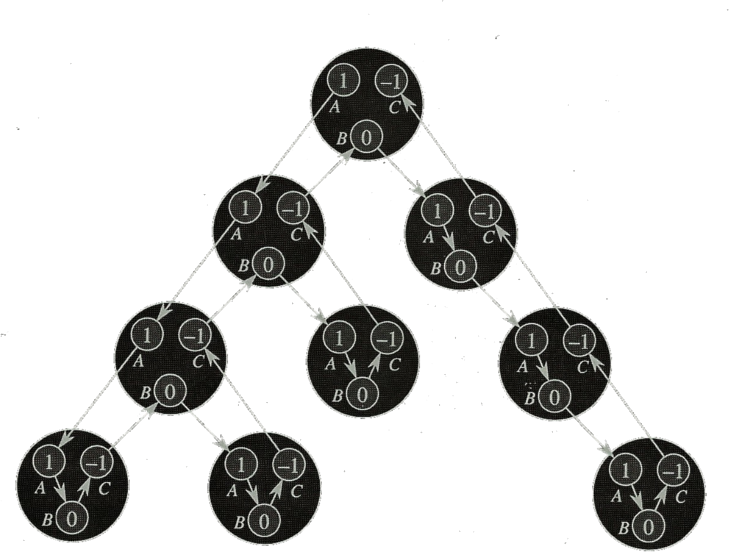
\includegraphics[width=8cm]{euler1.png}
  \end{center}

  \uncover<2>{Depth = prefix sum}
\end{frame}

\begin{frame}\frametitle{Graph Algorithms}
  \begin{itemize}
  \item
    depth-first visit
  \item
    No $\mathcal{NC}$ algorithm
  \item
    breadth-first visit
  \item
    $O(n^{2.37})$ processors
  \item
    \alert{Euler tour}
  \end{itemize}
\end{frame}

\begin{frame}\frametitle{Graph Algorithms}
  \begin{itemize}
  \item
    For each edge $e$, store its successor $s(e)$
  \item
    Euler tour of $G$ = edge-disjoint cycles
  \item
    merge any two cycles with a common vertex $u$
  \end{itemize}
\end{frame}

\begin{frame}\frametitle{Minimum Spanning Tree (MRC)}
  \begin{algorithm}[H]
    \KwData{Array}{dense graph $G=\left\langle V,E \right\rangle $}

    \tcc{$|V|=n$, $|E|\ge n^{1+c}$}
    $V_{1}, \ldots, V_{k} \gets $ random balanced partition of $V$\;
    $E_{i,j} \gets \{(u, v) \in E | u, v \in V_{i} \cup V_{j} \}$\;
    $G_{i,j} \gets $ subgraph of $G$ induced by $E_{i,j}$\;
    \ForEach{$G_{i,j}$}{
      $M_{i,j}\gets $ minimum spanning forest of $G_{i,j}$
    }
    $H \gets \left\langle V, \bigcup_{i,j} M_{i,j}\right\rangle $\;
    $M \gets$ minimum spanning tree of $H$\;
    \label{alg:MRC-MST}
    \caption{MST}
  \end{algorithm}
\end{frame}

\begin{frame}\frametitle{Minimum Spanning Tree (MRC)}
  \begin{block}{MST Algorithm is correct}
    \begin{enumerate}
      \item
    Let $e\in E\setminus E(H)$.
      \item
    Then $e$ is a heaviest edge in some cycles of $G_{i,j}$.
      \item
    The same cycle is also in $G$.
  \end{enumerate}
\end{block}
\end{frame}


\begin{frame}\frametitle{Connected components}
  \begin{algorithm}[H]
    Label each vertex either \alert{up} or \alert{down}\;
    \ForEach{edge $(v,w)$}{
      Add the component of the down vertex to that of the up vertex\;
      \tcc{The root of the lower component is now a child of the root of the
        upper component}
    }
    \ForEach{vertex $v$}{
      parent[$v$] $\gets$ parent[parent[$v$]]
    }
    \caption{ConnectedComponents}
  \end{algorithm}
\end{frame}

\begin{frame}\frametitle{Additional Bibliography on PRAM}
  \small
   Parallel Computing PRAM Algorithms
   \url{http://www.cs.unc.edu/~prins/Classes/633/Handouts/pram.pdf}

A Survey of Parallel Algorithms for Shared-Memory Machines
\url{http://techreports.lib.berkeley.edu/accessPages/CSD-88-408.html}
\end{frame}


\end{document}

%%% Local Variables:
%%% mode: latex
%%% TeX-PDF-mode: t
%%% buffer-file-coding-system: utf-8
%%% End:
